\clearpage
\section{Cautionary Tale on Filtering}
\label{filtering}

It is tempting to insert standard filtering techniques from signal processing 
after creating a Gaussian process model but prior to any DTW or contribution 
calculations. A fast Fouier transform (FFT) \citeme based low-pass filter or 
Mel-frequency cepstral coefficients (MFCC) \citeme could be used to reduce error 
in the model itself, 
and thus make the contribution measure more precise. Unfortunately, most 
fuel cycle metrics are not well-formed candidates for such filtering strategies.
Including such filters as part of the analysis can easily lead to wildly unphysical
models.

Consider a simple low-pass filter where a 256 channel real-valued FFT frequency 
transform is taken.  All but lowest 32 channels are discarded prior to the applying 
the inverse transform. High frequency jitter in the original signal is removed, 
allowing for a better signal-to-noise ratio.

\begin{figure}[htb]
\centering
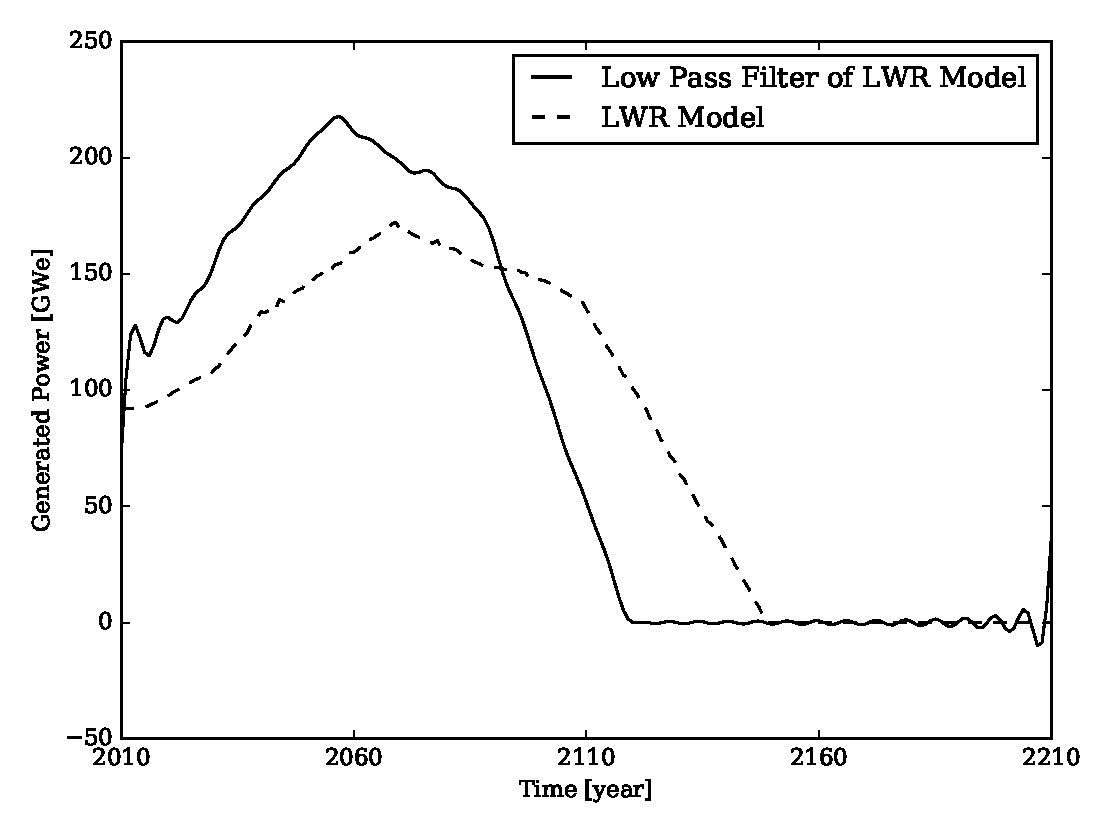
\includegraphics[width=0.45\textwidth]{fft-lwr-model.eps}
\caption{Low-pass FFT filter of LWR Gaussian process model $m_*^\LWR$ alongside
the unfiltered model model.}
\label{fft-lwr-model}
\end{figure}

Figure \ref{fft-lwr-model} shows the results of applying the low-pass filter 
described above to the Gaussian process model of the generated power from LWRs, 
$m_*^\LWR$.  The filtered curve demonstates at least three major problems.  The
first is that the values of the curve are allowed to be negative, which is 
impossible for this (and many other) fuel cycle metric.  The second is that 
near the time boundaries ($t=2010$ and $t=2210$), the amplitude of the filtered model
is significantly higher than itself. At $t=2210$, the metric should be zero but
instead is 36.5 GWe. Thirdly, the shape of the curve itself is skewed to lower 
times. The time at which the metric goes to zero should be near year 2150 but is 
instead closer to year 2115.  All of these issues would severly distort any 
DTW calculations that follow.

The reason behind these inconsistencies is that the FFT process is fundemenatally 
periodic.  However, using the annual time grid here, most fuel cycle metrics 
are not periodic. Neither is the modeling error for such metrics periodic. 
Thus, while well-intentioned, a low-pass filter is not generally applicable.

Alternatively, MFCCs provide a mechanism for converting a time series into a 
set of power spectrum coefficient curves. Since the dynamic time warping procedure
uses an L1 norm to form the cost matrix, the MFCCs of two signals can be directly 
compared. Each coefficient should roughly correspond in shape and amplitude to some
feature in the original signal.  Noisy, high frequency coeffients tend to be 
very similar and so their contribution to a DTW is less cooresponding less than 
lower coefficients. Coupling MFCC to DTW is an extremely common method employeed in 
speech recognition systems.  


Recomended to pick a different kernel instead.